\chapter{Serving models and architectures}
\label{ch:serving-and-architecture}

\section{Architectures by recommendation structure}

We have returned several times to the concept of Collector, Ranker, Server, and we've seen that those may be considered via two paradigms: the online and the offline modes. Further, we've seen how many of the components in the last chapter on data processing satisfy some of the core requirements of these functions.

In designing large systems like these, there are a number of architectural considerations. Now we'd like to demonstrate how these concepts adapt based on the type of recommendation system you are building. For this purpose we compare a mostly standard item-to-user recommendation system, a query-based recommendation system, contextual recommendations, and sequence-based recommendations.

\subsection{Item-to-user recommendations}

First up is the system we've been discussing thus far! As proposed in [4 System Design for Recommendation Systems](https://www.notion.so/4-System-Design-for-Recommendation-Systems-adfc961643194fa295c799ac2dfc300e), we build the collector offline to ingest and process our recommendations. We utilize representations to encode relationships between items, users, or user-item pairs. The online collector takes the request, usually in the form of a user-id, and finds a neighborhood of items in this representation space to pass along to the ranker. Those items are filtered when appropriate and sent for scoring. The offline ranker trains the relevant features for scoring and ranking, training on the historical data. The online ranker uses this model and potentially the necessary features for inference. In the case of recommendation systems this inference is the scores associated to each item in the set of potential recs. We usually sort by this score. Finally, we integrate a final round of ordering based on some business logic. This last step is part of the serving where we impose things like test-criteria or recommendation diversity requirements.

\begin{figure}[h!]
    \caption{This image by Karl Higley and Even Oldridge is an excellent overview of the architecture we've just described. (used with permission)}
    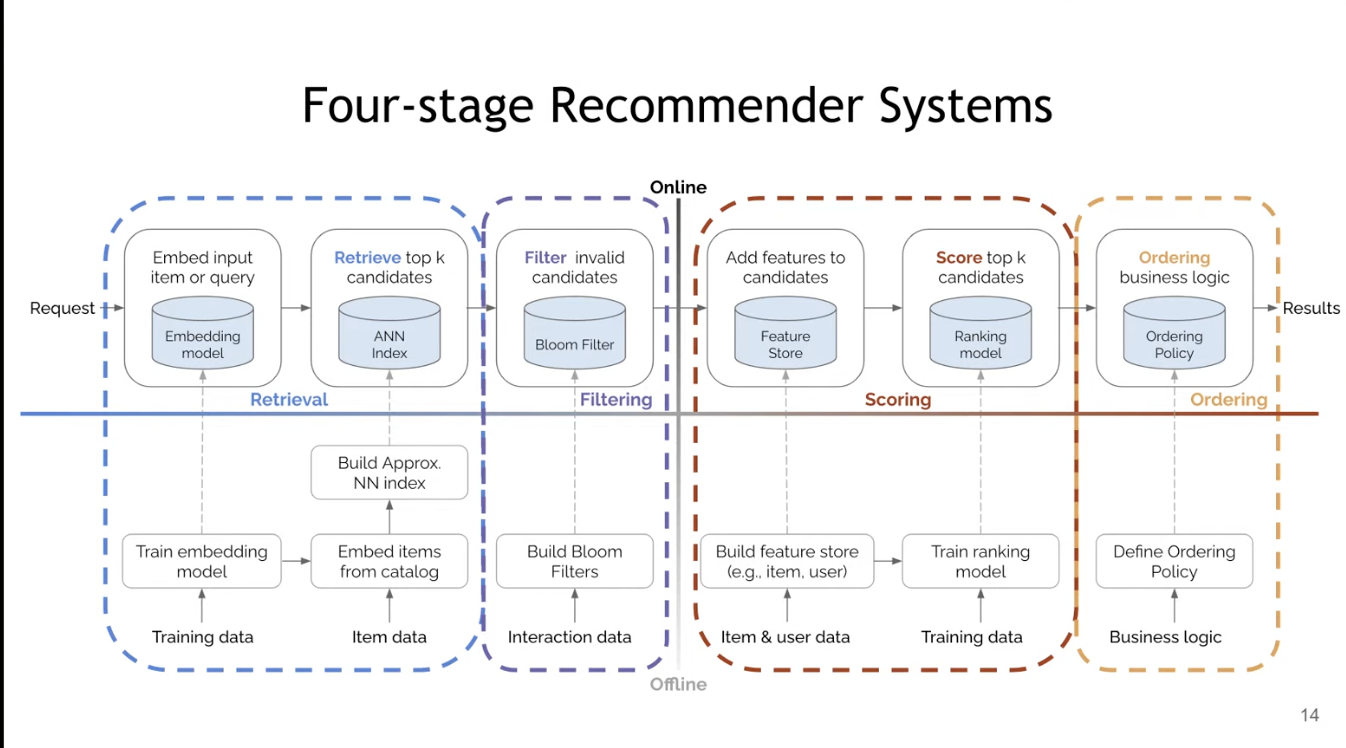
\includegraphics[width=\textwidth-10pt]{book-text/four-stage-diagram.png}
\end{figure}

\subsection{Query-based recommendations}

Next we want to include a query to start off our process. The most obvious example of a query is a text query like in text-based search engines. However, queries may be more general! For example you may wish to allow search-by-image, or search-by-tag. While these systems are quite similar in overall structure to the above, let's discover how to modify them to fit our use-case.

Immediately, we wish to integrate something more into the first step of the request. Note that we don't want to throw out the user-item matching components of this system\textemdash even though the user is performing a search, there's utility in personalizing the recommendations based on their taste. So now we need to utilize the query in addition; later we will discuss various technical strategies, but a simple summary for now is to also train an embedding for the query! Note that the query is like and item, but sufficiently different. Some strategies might include similarity between the query and items, or co-occurrence of the query and items. Either way, we now have a query representation and user-representation, and we want to utilize both for our recommendation. One simple strategy here is to use the query representation for retrieval, but during the scoring, score via both query-item and user-item, combining them via a multi-objective loss. Another strategy is to use the user for retrieval, and then the query for filtering. 

\subsection{Context-based recommendations}

A context is actually quite similar to a query, but tends to be more obviously feature based. Context is usually the term use to represent some exogenous features to the system, that may have an effect on the system, i.e. auxiliary information such as time, weather, location, and more. The ways in which it is similar to query-based recommendation are that it's an additional signal that the system needs to consider during recommendation, but more often than not: query should dominate the signal for recommendation, whereas context should not. 

Let's take a simple example: when ordering food. A query for a food-delivery recommendation system would look like 'Mexican food'; an extremely important signal from the user of how the recs should look. A context for a food-delivery recommendation system would look like 'it's almost lunch time'; a useful signal, but either equally weighted with user-personalization or lesser. It's hard to put hard and fast rules on this weighting, so usually we don't, and just learn parameters via experimentation.

How they fit into the architecture is very similar to queries, but via these features. Learn a representation between context features and items, and add that affinity into the rest of the pipeline. Again you can make use of this early in the retrieval, later in the ranking, or even during the ordering step. 

\subsection{Sequence-based recommendations}

Sequence based recommendations builds on context-based recommendations, but with a specific type of context. Sequential recommendations are the concept that the lagging items the user has been exposed to should have a significant influence on the recommendations. A common example here is a music streaming service, where the last few songs that have been played can significantly help inform what the user might want to hear next. To ensure this 'auto-regressive' set of features has an influence on recommendations, we can treat each item in the sequence as a weighted context for the recommendation.

Usually, the item-item representation similarities are weighted to provide a collection of recommendations and various strategies are used for combining these. In this case, we normally expect the user to be of high importance in the recommendations but the sequence is also of high importance. One simple model is to think of the sequence of items like a sequence of tokens, and form a single embedding for that sequence\textemdash like in NLP applications. This embedding can be used as the context in a context-based recommendation architecture.

\subsection{Aside: Why bother with extra features}

Sometimes it is useful to step back and ask if a new technology is actually worth caring about. So far in this section we've introduce four new paradigms for how to think about a recommender problem. That may seem surprising and potentially even unnecessary. 

One of the core reasons that things like context and query based recommendations become relevant is to deal with some of the issues mentioned before around sparsity and cold-starting. Sparsity makes things that aren't cold seem cold via the learner's under-exposure to them, but true cold starting also exists due to new items being added to catalogs all the time in most applications. We will address cold-starting in detail, but for now, suffice to say that one strategy for warm starting is to use other features which *are* available even in this regime.

In applications of machine learning that are explicitly feature based, we rarely battle the cold-start problem to such a degree, because at inference time we're confident that the model parameters useful for prediction are well aligned with those features that are available. In this way, feature-included recommendation systems are bootstrapping from a potentially weaker learner, that has more guaranteed performance via always available features. 

The second analogy that the previous architectures are reflecting is that of boosting. Boosted models operate via the observation that ensembles of weaker learners can reach better performance. Here we are asking for some additional features to help these networks ensemble with weak learners, to boost their performance. 

\section{Encoder architectures \& cold starting}

The previous problem framings of different types of recommendation problems points out four model architectures, each fitting into our general framework of collector, ranker, server; now let's discuss in a bit more detail how model architecture can become intertwined with serving architecture. In particular, we also wish to discuss feature encoders. 

The key opportunity from encoder-augmented systems is that for users, items, or contexts without much data, we can still form embeddings on the fly. Recall from before that our embeddings made the rest of our system possible, but cold-starting recommendations was a huge problem.

The \emph{two-towers architecture}\textemdash \emph{or dual encoder networks}\textemdash introduced in [Yi et. al.]\url{https://storage.googleapis.com/pub-tools-public-publication-data/pdf/6c8a86c981a62b0126a11896b7f6ae0dae4c3566.pdf}, is an explicit model architecture aimed at prioritizing features of both the user and items, when building a scoring model for a recommendation system. Our previous discussion of matrix factorization described it as a collaborative filter, focused on utilizing implicit similarity via interaction to provide our affinities. From last section, it is now obvious to you that additional features matter. While adding these \emph{side-car} features into a matrix factorization paradigm is possible and has shown to be successful, c.f. [[CF for Implicit Feedback]\url{http://yifanhu.net/PUB/cf.pdf}, [Factorization Machines]\url{https://www.csie.ntu.edu.tw/~b97053/paper/Rendle2010FM.pdf}, [SVDFeature]\url{http://wnzhang.net/papers/svdfeature-jmlr.pdf}, in this model we will take a more direct approach. 

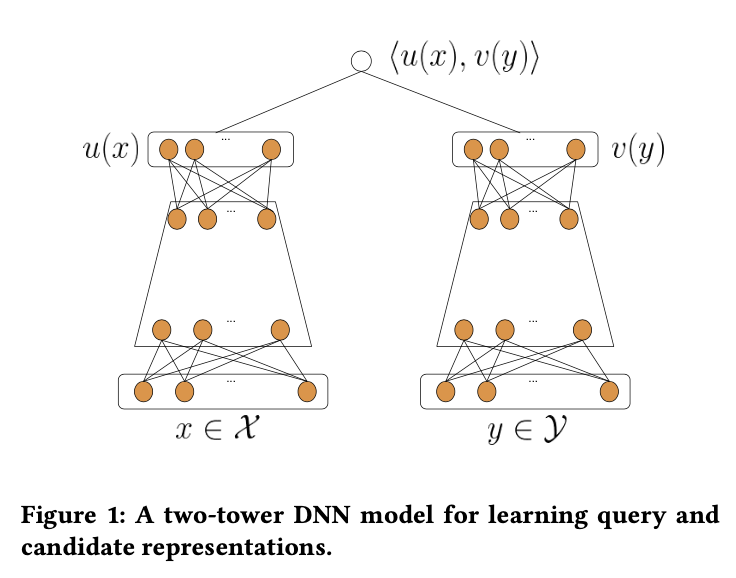
\includegraphics[width=\textwidth-10pt]{book-text/two-towers-architecture-diagram.png}

In this architecture, we take the left tower to be responsible for items, and the right tower to be responsible for user\textemdash and when appropriate\textemdash context. These two tower architectures are inspired from the NLP literature and in particular the [Learning Text Similarity](https://aclanthology.org/W16-1617.pdf) work. 

Let's work through in detail how this model architecture is applied to recommending videos on YouTube. Note that this follows the paper introducing this architecture. Training labels will be given by clicks, but with an additional regression feature $r_i\in [0,1]$ where the minimum value corresponds to click but trivial watch-time, and the maximum of the range corresponds to a full-watch. 

As mentioned above, this model architecture will explicitly include features from both user and items. The video features will consist of categorical and continuous features, like \lstinline{VideoId}, \lstinline{ChannelId}, \lstinline{VideoTopic}, and so on. An embedding layer is used for many of the categorical features to move to dense representations. The user features are things like watch histories via bag of words, and standard user features.

This model structure combines many of the ideas we've seen before, but has relevant takeaways for our system architecture. First, is the idea of sequential training. Each 'temporal batch' of samples, should be trained in sequence to ensure that model drift is shown to the model. Next, we see an important idea for the productionizing of these kinds of models:  encoders.

In these models, we have feature encoders as the early layers in both towers, and when we move to inference, we will still need these encoders. When performing the online recommendations, we will be given \lstinline{user_id} and \lstinline{video_id}, and first need to collect their features. As discussed before, the Feature Store will be useful in getting these raw features, but we need to also encode into the dense representations necessary for inference. This is something that can be stored in the feature store for known entities, but for unknown entities we will need to do the feature embedding at inference time.

Encoding layers serve as a simple model for mapping a collection of features to a dense representation. When fitting encoding layers as the first step in a neural network, the common strategy is to take the first $k$ layers and re-use them as an encoder model. More specifically, if $\mathcal{L}^i, 0\leq i\leq k$ are the layers responsible for feature encoding, call $Emb(\hat{V})=\mathcal{L}^k(\mathcal{L}^{k-1}(\ldots\mathcal{L}^0(\hat{V})))$ the function which maps a feature vector $\hat{V}$, to it's dense representation.

In our previous system architecture, we would include this encoder as part of the fast layer, after receiving features from the feature store. It's also important to note that we would still want to utilize vector search; these feature embedding layers are used upstream of the vector search and nearest neighbor searches.

\section{Deployment}

Like many applications of Machine Learning, the final output of a recommendation systems is itself a small program that runs continuously and exposes an API to interact with it. In much of what we've already done this chapter, we've seen the pieces embedded in that system, but now we should discuss the components closer to the user. 

In our relatively general architecture, the server is responsible for handing over the recommendations, after all the work that comes before and it should adhere to a preset schema. But what does this deployment look like?

\subsection{Models as APIs}

Let's discuss two systems architectures that might be appropriate for serving your models in production: micro-service and monolith.

In web applications this dichotomy is well covered from many perspective and special use-cases. As ML engineers, Data Scientists, and potentially Data Platform engineers, it's not necessary to dig deep into this area, but it's essential to know the basics. Simply: \emph{micro-service architectures} state that each component of the pipeline should be it's own small program with clear API and output schema, composing these API calls allow for flexible and predictable pipelines. In contrast, \emph{monolithic architectures} suggest that one application should contain all the necessary logic and components for model predictions, keeping the application self-contained means less interfaces that need to be kept aligned and less rabbit holes to hunt in when some location in your pipeline is being starved.

Whatever you choose as your strategy, you'll need to make a few decisions:

\begin{itemize}
\item How large is the necessary application? If your application will need fast access to large dataset at inference time, you'll need to think carefully about memory requirements.
\item What access does your application need? We've previously discussed making use of things like Bloom filters, and Feature stores; these resources may be tightly coupled to your application\textemdash by building them in memory in the application\textemdash or they might be an API call away. Make sure your deployment accounts for these relationships.
\item Should your model be deployed to a single node or a cluster? For some types of model, even at the inference step we wish to utilize distributed computing. This will require additional configuration to allow for fast parallelization.
\item How much replication do you need? \emph{Horizontal scaling} allows you to have multiple copies of the same service running simultaneously to reduce the demand on any particular instance. This is important for ensuring availability and performance. As we horizontally scale, each service can operate independently and there are different strategies for coordinating these services and an API request. Each replica is usually it's own containerized application and things like CoreOS and Kubernetes are used to manage these. The requests themselves must also be balanced to the different replicas via something like NGINX.
\item What are the relevant API's exposed? Each application in the stack should have a clear set of exposed schemas, and an explicit communication about what types of other applications may call to them.
\end{itemize}

\paragraph{Spinning up a model service}

So what can you use to actually get your model into an application? One of a variety of frameworks for application development are useful; some of the most popular in Python are Flask, FastAPI, and Django. Each have different advantages, but we'll choose to discuss here FastAPI. 

FastAPI is a targeted framework for API applications, making it especially well fit for serving ML models. It calls itself an ASGI (Asynchronous Server Gateway Interface) framework; and it's specificity grants a ton of simplicity. 

Let's take a simple example of turning a fit torch model into a service with the FastAPI framework. First, let's utilize an artifact store to pull down our fit model; here we are using Weights and Biases artifact store:


\begin{lstlisting}[language=python]
import wandb, torch
run = wandb.init(project=Prod_model, job_type="inference")

model_dir = run.use_artifact(
		'bryan-wandb/recsys-torch/model:latest', 
		type='model'
).download()

model = torch.load(model_dir)
model.eval(user_id)
\end{lstlisting}

This looks just like your notebook workflow, so let's see how easy it is to integrate this with FastAPI:

\begin{lstlisting}[language=python]
from fastapi import FastAPI # FastAPI code

import wandb, torch

app = FastAPI() # FastAPI code

run = wandb.init(project=Prod_model, job_type="inference")

model_dir = run.use_artifact(
	'bryan-wandb/recsys-torch/model:latest', 
	type='model'
).download()

model = torch.load(model_dir)

@app.get("/recommendations/{user_id}") # FastAPI code
def make_recs_for_user(user_id: int): # FastAPI code
		endpoint_name = 'make_recs_for_user_v0'
		logger.info(
			"{'type': 'recommendation_request'," 
			f"'arguments': {'user_id': {user_id}}," 
			f"'response': {None}},",
			f"'endpoint_name': {endpoint_name}"
		)
		recommendation = model.eval(user_id)
		logger.log(
			"{'type': 'model_inference'," 
			f"'arguments': {'user_id': {user_id}}," 
			f"'response': {recommendation}},"
			f"'endpoint_name': {endpoint_name}"
		)
    return { # FastAPI code
			"user_id": user_id, 
			"endpoint_name": endpoint_name, 
			"recommendation": recommendation
		}
\end{lstlisting}

I cannot stress enough that via only we now have a model-as-a-service in five additional lines of code. We will see more discussion about logging later to help you improve observability in all of your applications, but here I included some very simple examples of logging. 

\section{Alerting and Monitoring}

Alerting and monitoring take a lot of their inspiration from the DevOps world for software engineering. Some high level principles which will guide our thinking are:

\begin{itemize}
\item clear defined schemas and priors
\item observability
\end{itemize}

\subsection{Schemas and Priors}

When designing software systems, you almost always have expectations of how the components fit together. Much like in writing code you anticipate the input and output to functions, in software systems you anticipate these at each interface. Not only for micro-service architectures is this relevant; even in a monolith architecture components of the system need to work together and often will have boundaries between their defining responsibilities. 

Let's make this more concrete via an example: you've built a user-item latent space, a feature store for user features, a bloom filter for client avoids, and an experiment index which defines which of two models should be used for scoring. First let's examine the latent space: when provided a \lstinline{user_id} we need to look up its representation, and we have some assumptions already:

\begin{itemize}
\item \lstinline{user_id} provided will be of the correct type
\item \lstinline{user_id} will have a representation in our space
\item The representation returned will be of the correct type and \lstinline{shape}
\item The component values of the representation vector will be in the appropriate domain. \emph{(Note: the support of representations in your latent space may vary day-to-day)}
\end{itemize}

From here, we need look up the $k$ Approximate Nearest Neighbors, which incurs more assumptions:

\begin{itemize}
\item There are $\geq k$ vectors in our latent space
\item Those vectors adhere to the expected distributional behavior of the latent space
\end{itemize}

While these seem relatively straightforward application of unit-tests, canonizing these assumptions is important. Take the last assumption in both of the two services: how can you know the appropriate domain for the representation vectors? As part of your training procedure, you'll need to calculate this, then store it for access during the inference pipeline. 

In the second case, when finding nearest neighbors in high dimensional spaces, there are well discussed difficulties in distributional uniformity, but this can mean particularly poor performance for recommendations. In practice, the authors have observed a spiky nature to the distribution of $k$-NN in latent spaces, leading to difficult challenges downstream in ensuring diversity of recommendations. These distributions can be estimated as priors and simple checks like KL-divergence can be used online. 

In both cases, collecting the output of this information and logging it can provide a rich history of what is going on with your system; this can shorten debugging loops later on if model performance is low in production.

Returning to the possibility of \lstinline{user_id} lacking a representation in our space: this is precisely the cold-start problem! In that case we need to transition over to a different prediction pipeline: perhaps user-feature-based, explore-exploit, or even hard-coded recommendations. In this setting, we need understand next steps when a schema condition is not met and gracefully move forward. 

\paragraph{Integration tests}

Let's consider one higher-level challenge that might emerge in a system like this at the level of integration. Some refer to these issues as \emph{entanglement.}

You've found through experimentation that you should find $k=20$ approximate nearest neighbors in the item-space for a user to get good recommendations. You make a call to your representation space, get your 20 items, and pass them onto the filtering step. However, this user is quite picky; they have previously made many restrictions on their account about what kind of recommendations they allow: no shoes, no dresses, no jeans, no hats, no handbags \textemdash what's a struggling RecSys to do! 

Naively, if you take the 20 neighbors, and pass them into the bloom, you're likely to be left with nothing! There are two ways to approach this challenge:

\begin{itemize}
\item allow for a call-back from the filter step to the retrieval
\item build a user-distribution and store that for access during retrieval
\end{itemize}

In the first of these, you give access to your filter step to call the retrieval step with a larger $k$ until the requirements are satisfied after the bloom. Of course, this incurs significant slow-down as it requires multiple passes and ever growing queries with redundancy! While this approach is simple, it requires building defensively and knowing ahead of time what may go wrong.

In the second of these, during training, you can sample from the user space to build estimates of the appropriate $k$ for varying numbers of avoids by user. Then giving access to a lookup of total avoids-by-user to the collector can help defend against this behavior.

\subsection{Observability}

There are quite a number of tools in the software engineering to assist with observability, understanding the why's of what's going on in the software stack. Because the systems we are building become quite distributed, the interfaces become critical monitoring points, but the paths also become complex.

Common terms in this area are \emph{spans} and \emph{traces,} which refer to two dimensions of a call stack. Given some collection of connected services, like in our above examples, an individual inference request will pass through some or all of those services in a sequence. The sequence of service requests is the trace. The, potentially parallel, time-delays of each of these services, is the span. 

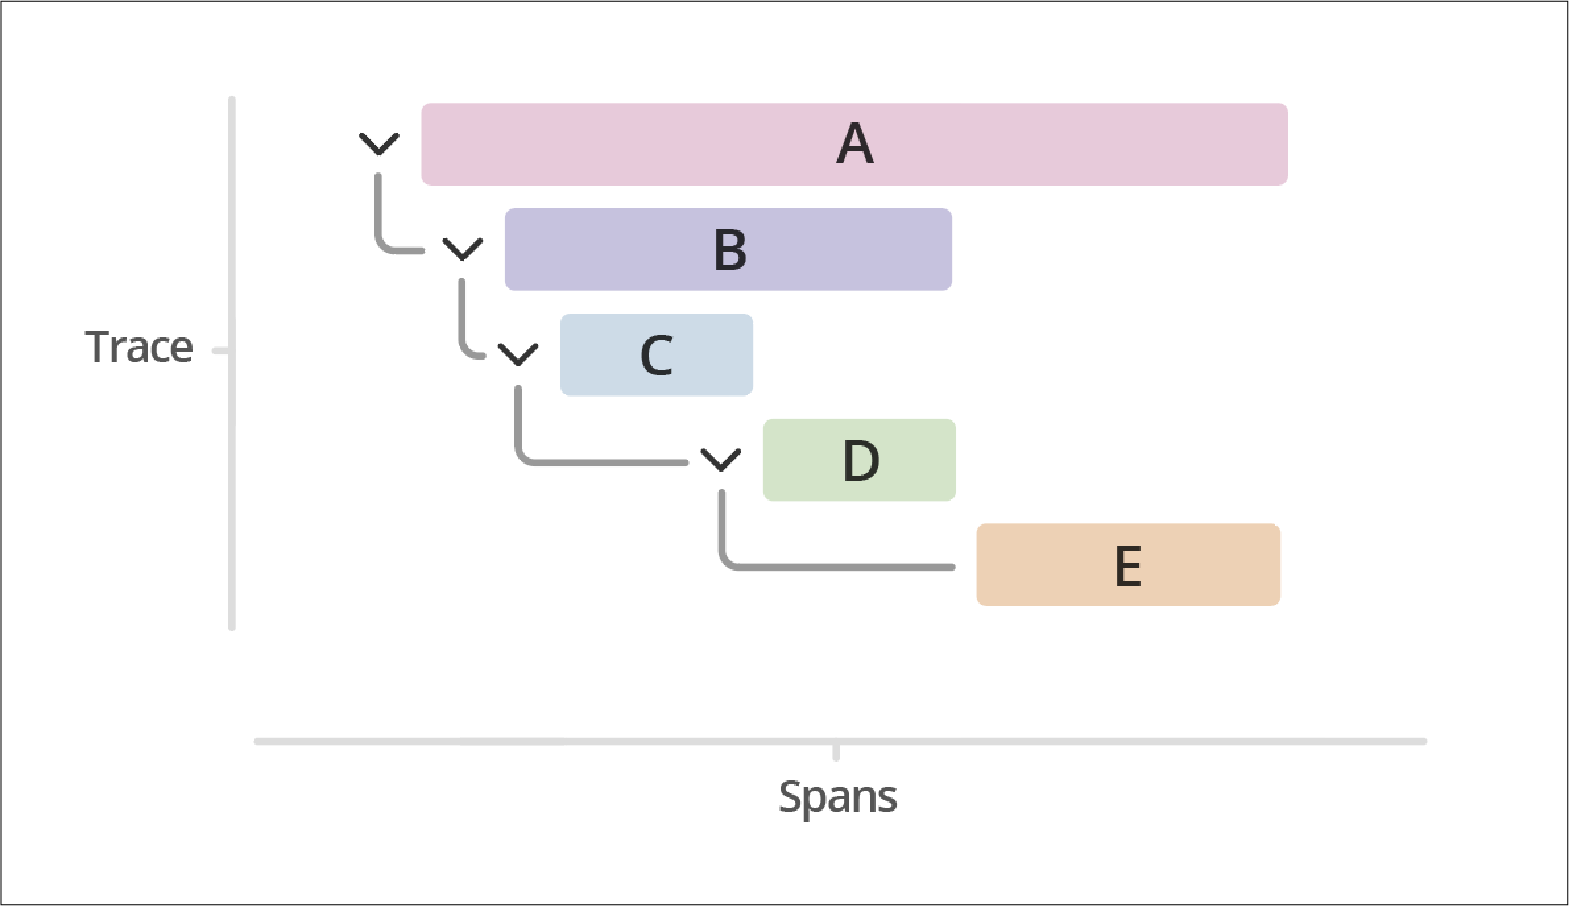
\includegraphics[width=\textwidth-10pt]{book-text/trace-spans.png}

The graphical representation of spans usually demonstrates how the time for one service to respond is comprised of several other delays from other calls. 

Observability is being able to see traces, spans, and logs in conjunction to appropriately diagnose the behavior of your system. In our example above where we utilize a call-back from the filter step to get more neighbors from the collector, we might see a slow response and wonder "what has happened?". By viewing the spans and traces, we'd be able to see that the first call to the collector was as expected, then the filter step made a call to the collector, then another call to the collector, and so on, which built up a huge span for the filter step. Combining that view with logging would help us rapidly diagnose what might be happening.

\paragraph{Time-outs}

In the above example, we had a long process that could lead to very bad user experience. In most cases, we impose hard restrictions on how bad we let things get; these are called time-outs. 

Usually we have an upper bound on how long we're willing to wait for our inference response, and so implementing time-outs aligns our system with these restrictions. It's important in these cases to have a \emph{fall-back.} In the setting of recommendation systems, a fall-back is usually comprised of things like the MPIM prepared such that it incurs minimal additional delay. 

\section{Evaluation in Prod}

If the previous section was understanding what's coming into your model in production, this might be summarized as what's coming out of your model in production. At a high level, evaluation in Prod can be thought of as extending all your model validation techniques to the inference time. In particular, *what the model actually is doing!*

On one hand we already have tools to do this evaluation \textemdash you can use the same methods used for evaluating performance as in training, but now on real observations streaming in. However, this is not as obvious as we might first guess.

\paragraph{Slow feedback}

Recommendation systems fundamentally are trying to lead to item selection, and in many cases, purchases. But if we step back and think more holistically about how recommendation systems integrate into businesses, it's to drive revenue. If you're an e-commerce shop, item selection and revenue may seem easily associated: a purchase leads to revenue, so good item recommendation leads to revenue. However, what about returns? Or even a harder question: are these revenue incremental? One challenge with recommendation systems, is there may sometimes be a very difficult to draw causal arrow between any metric used to measure the performance of your models to the business-oriented key performance indicators.

We call this slow feedback because sometime the loop to get from a recommendation, to a meaningful metric, and back to the recommender can take weeks or even longer. This is especially challenging when you want to run experiments to understand if a new model should be rolled out. The length of the test may need to stretch quite a bit more to get meaningful results. 

Usually a proxy metric is aligned on that the data scientists believe is a good estimator for the KPI, and that proxy metric is measured live. There are a huge variety of challenges with this approach, but it often suffices and provides motivation for more testing. 

\paragraph{Model metrics}

So what are the key metrics to track for your model in prod? Given that we're looking at recommendation systems at inference time, we should seek to understand:

\begin{itemize}
\item distribution of recommendation across categorical features
\item distribution of affinity scores
\item number of candidates
\item distribution of other ranking scores
\end{itemize}

As we discussed before, during the training process, we should be calculating broadly what the ranges of our similarity scores are in our latent space. While we can look at high level estimations, or finer ones, we can use these distributions to get warning signals something might be strange. Simply comparing the output of our model during inference, or over a set of inference requests, to these pre-compute distributions can be extremely helpful.

Comparing distributions can be a long topic, but one standard approach is \emph{KL-Divergence} between the observed distribution, and the expected distribution from training. By computing KL-Divergence between these, we can understand how 'surprising' the model's predictions are on a given day. 

What we'd really like is to understand the ROC of your model predictions with respect to one of your conversion types. However, this involves yet another integration to tie back to logging. Since your model API only produces the recommendation, you'll still need to tie into logging from the web application to understand outcomes! To tie back in outcomes one must join the model predictions with the logging output to get the evaluation labels, which can be done via log parsing technologies (like ELK or Prometheus). We'll see more of this in the next chapter. 

\section{Continuous training and deployment}

It may feel like we're done with this story since we have models tracked and production monitoring in place, but rarely are we satisfied with set-it-and-forget-it of model development. One important characteristic of ML products, is how models frequently need to be updated to even be useful. Above we discussed model metrics, and how sometimes performance in production might look different than what we had come to expect from the trained models' performance. This can even be further exacerbated by \emph{model drift.}

Model drift is the notion that the same model may exhibit different prediction behavior over time, merely due to changes in the data generating process. A very simple example is a time-series forecasting model. When you build a time-series forecast model, the specially unique property that is essential for good performance is \emph{auto-regression,} that is to say that the value of the function covaries with previous values of the function. We wont go into detail on time-series forecasting, but suffice to say: the best hope you have of making a good forecast is to use up-to-date data! If you wanted to forecast stock prices, you'd always want to use the most recent prices as part of your predictions. This simple example demonstrates how models may drift; a model that did well two weeks ago, needs to be retrained with recent data to be expected to continue to perform well.

One criticism of a model that drifts is "that's the smoking gun of an overfit model", but in reality these models require a certain amount of over-parameterization to have useful models. In the context of recommendation systems, we've already seen things like the Matthew Effect can have disastrous effects on the expected performance of a recommender model. If we don't consider thinks like new items in our recommender, we are doomed to fail. Models can drift for a variety of reasons, often coming down to exogenous factors in the generating process that may not be captured by the model. 

One approach to dealing with and predicting stale models, is to simulate these scenarios during training. If your expectation is that the model goes stale mostly due to the distribution changing over time, you can employ sequential cross-validation \textemdash  i.e. train on a contiguous period and test on a subsequent period \textemdash but with a specified block of time delay. For example, if you think your model performance is going to decrease after two week due to being trained on out-of-date observations, then during training you can purposely build your evaluation to incorporate a two-week delay before measuring performance. This is called \emph{two-phase prediction comparison} and by comparing the performances you can estimate drift magnitudes to keep an eye out in prod. 

There are a wealth of statistical approaches to reigning in these differences; in lieu of a deep dive into variational modeling for variability and reliability for your predictions, we'll instead discuss continuous training and deployment and open this peanut with a sledge hammer.

\subsection{Deployment topologies}

Let's consider a few different structures for how you want to deploy models to not only keep your models well in tune, but to accommodate iteration, experimentation, and optimization.

\paragraph{Ensembles}

Ensembles are a type of model structure in which multiple models are built, and the predictions from those models are pooled together in one of a variety of ways. While this notion of an ensemble is usually packaged into the model called for inference, you can actually generalize the idea to your deployment topology. Let's take an example that builds on our previous discussion of prediction priors. If we have a collection of models with comparable performance on a task, we can deploy them in ensemble weighted by their deviation from the prior distributions of prediction that we've set before. This way, instead of having a simple yes/no filter on the output of your model's range, you can more smoothly transition potentially problematic predictions into more expected ones. 

Another benefit of treating the ensemble as a deployment topology instead of only a model architecture, is that you can 'hot-swap' components of an ensemble as you make improvements in specific sub-domains of your observation feature space. Take for example an LTV model comprised of three components, one that predicts well for new clients, another for activated clients, and a third for super-users. You may find that pooling via a voting mechanism on average performs the best, so you decide to implement a bagging approach. This works well, but later you find a better model for the new clients. By using deployment topology for your ensemble you can swap in the new model for the new clients, and start comparing performance in your ensemble in prod. This brings us to the next strategy, model comparison.

\paragraph{Shadowing}

Deploying two models, even for the same task, can be enormously informative. We call this shadowing in the case where one model is "live" and the other is secretly also receiving all the requests and doing inference, and logging the results of course. By shadowing traffic to the other model, you get the best expectations possible about how the model behaves before making your model live. This is especially useful when wanting to ensure that the prediction ranges align with expectation. 

In software engineering and devOps, there's a notion of \emph{staging} for software. It's a hotly contested question of "how much of the real infra should staging see", but shadowing is the staging of ML models. You can basically build a parallel pipeline for your entire infrastructure to connect for shadow models, or you can just put them both in the line of fire and have the request sent to both, but only use one response. Shadowing is also crucial for implementing experimentation.

\paragraph{Experimentation}

As good data scientists, we know that without a proper experimental framework, it's risky to advertise much about the performance of a feature or in this case model. Experimentation can be handled with shadowing by having a controller layer that is taking the incoming requests and orchestrating which of the deployed models to curry the response along from. A simple A/B experimentation framework might ask for a randomization at every request, where-as something like a multi-armed bandit will require the controller layer to have notions of the reward function.

Experimentation is a deep topic which we don't have the knowledge or space to do adequate justice, but it's useful to know that this is where experimentation can fit into the larger deployment pipeline.

\paragraph{Aside: Model Cascades}

A really nice extension of several of the ideas is one of \emph{Model Cascading.} The simplified idea of a model cascade is that we use model confidence to create a conditional ensemble. In particular, given an inference request the model provides a prediction with a confidence estimate; when the model confidence is high that prediction is returned, but if the confidence is below some threshold, a downstream model is called and the ensemble is started. There's no reason to stop at two, for any number of models that in training show improved performance in ensemble, this method can be used to iteratively expand the number of ensemble layers. 

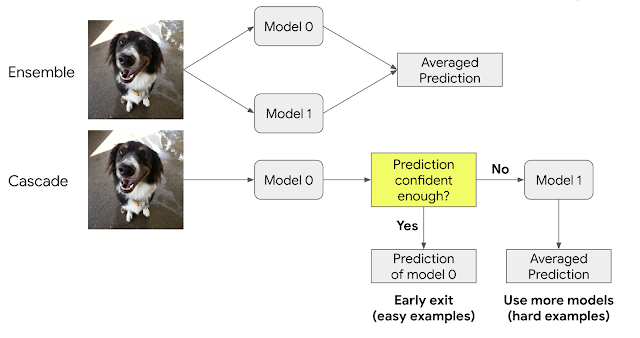
\includegraphics[width=\textwidth-10pt]{book-text/model-cascades.png}

A few advantages of this approach are:

\begin{itemize}
\item better expected performance overall; ensembles usually increase performance
\item ensemble performance with lower average computation time
\item especially better performance in out-of-sample scenarios
\end{itemize}

This method scales to larger pools of models and while it may incur significant training efforts, finding the right ordering of the models can have significant effects on model accuracy and latency.